\section{Results} \label{sec:results}

Figure~\ref{fig:glimit} shows the 95\% C.L. limits on \gagg\ and the ratio of the 95\% C.L. limits on \ggamma\ 
with respect to the KSVZ benchmark value ($\left|g_\text{KSVZ}\right|=0.97$).  
The blue error band indicates the systematic uncertainties as discussed in 
Sec.~\ref{sec:sys}. Note the uncertainties here are solely due to the 
variations in the experimental parameters and in the analysis procedure 
of TASEH; the uncertainties on the local dark matter density $\rho_a$,
 which can be as large as 50\%, are considered external uncertainties 
and not included in the blue error band.  
No limits are placed for the frequency ranges  
%4.710170 -- 4.710190~GHz and 4.747301 -- 4.747380~GHz, which correspond to 
4.71017 -- 4.71019~GHz and 4.74730 -- 4.74738~GHz, corresponding to 
the regions in which non-axion signals were observed 
during the collection of the CD102 data. The limits on 
\gagg\ range from \lolimit\GeVinv\ to \hilimit\GeVinv, with an average 
value of \avelimit\GeVinv; the lowest value comes from the frequency bins with 
additional eight times more data from the rescans, while the highest value 
comes from the frequency bins near the boundaries of the spectrum. 
Figure~\ref{fig:gaggall} displays the \gagg\ limits obtained by TASEH 
together with those from the previous searches. 
The results of TASEH exclude the models with the axion-two-photon coupling 
$\gagg\gtrsim \avelimit\GeVinv$, a factor of eleven above the benchmark
KSVZ model for the mass range $\mlo < \ma < \mhi \muevcc$ (corresponding to 
the frequency range of $\flo < f_a < \fhi$~GHz). 


The central results in Figs.~\ref{fig:glimit}--\ref{fig:gaggall} are 
obtained assuming an axion signal line shape that follows 
Eq.~\eqref{eq:simplesignal}. The \gagg\ limits from the analysis that merges 
frequency bins without 
assuming a signal line shape 
are $\approx5.5$\% larger than the central values. 
If a Gaussian signal line shape with an FWHM of 2.5~kHz,  
about half of the axion line width in Eq.~\eqref{eq:simplesignal}, is 
assumed instead, the limits will be $\approx3.8$\% smaller than the central 
results. 
If the \gagg\ limits are derived from the observed SNR as described in the 
ADMX paper~\cite{ADMXVIII}, 
rather than using the 5$\sigma$ target SNR, the average limit on \gagg\ will 
be $\approx\ADMXavelimit\GeVinv$. 


\begin{figure*} [htbp]
  \centering
  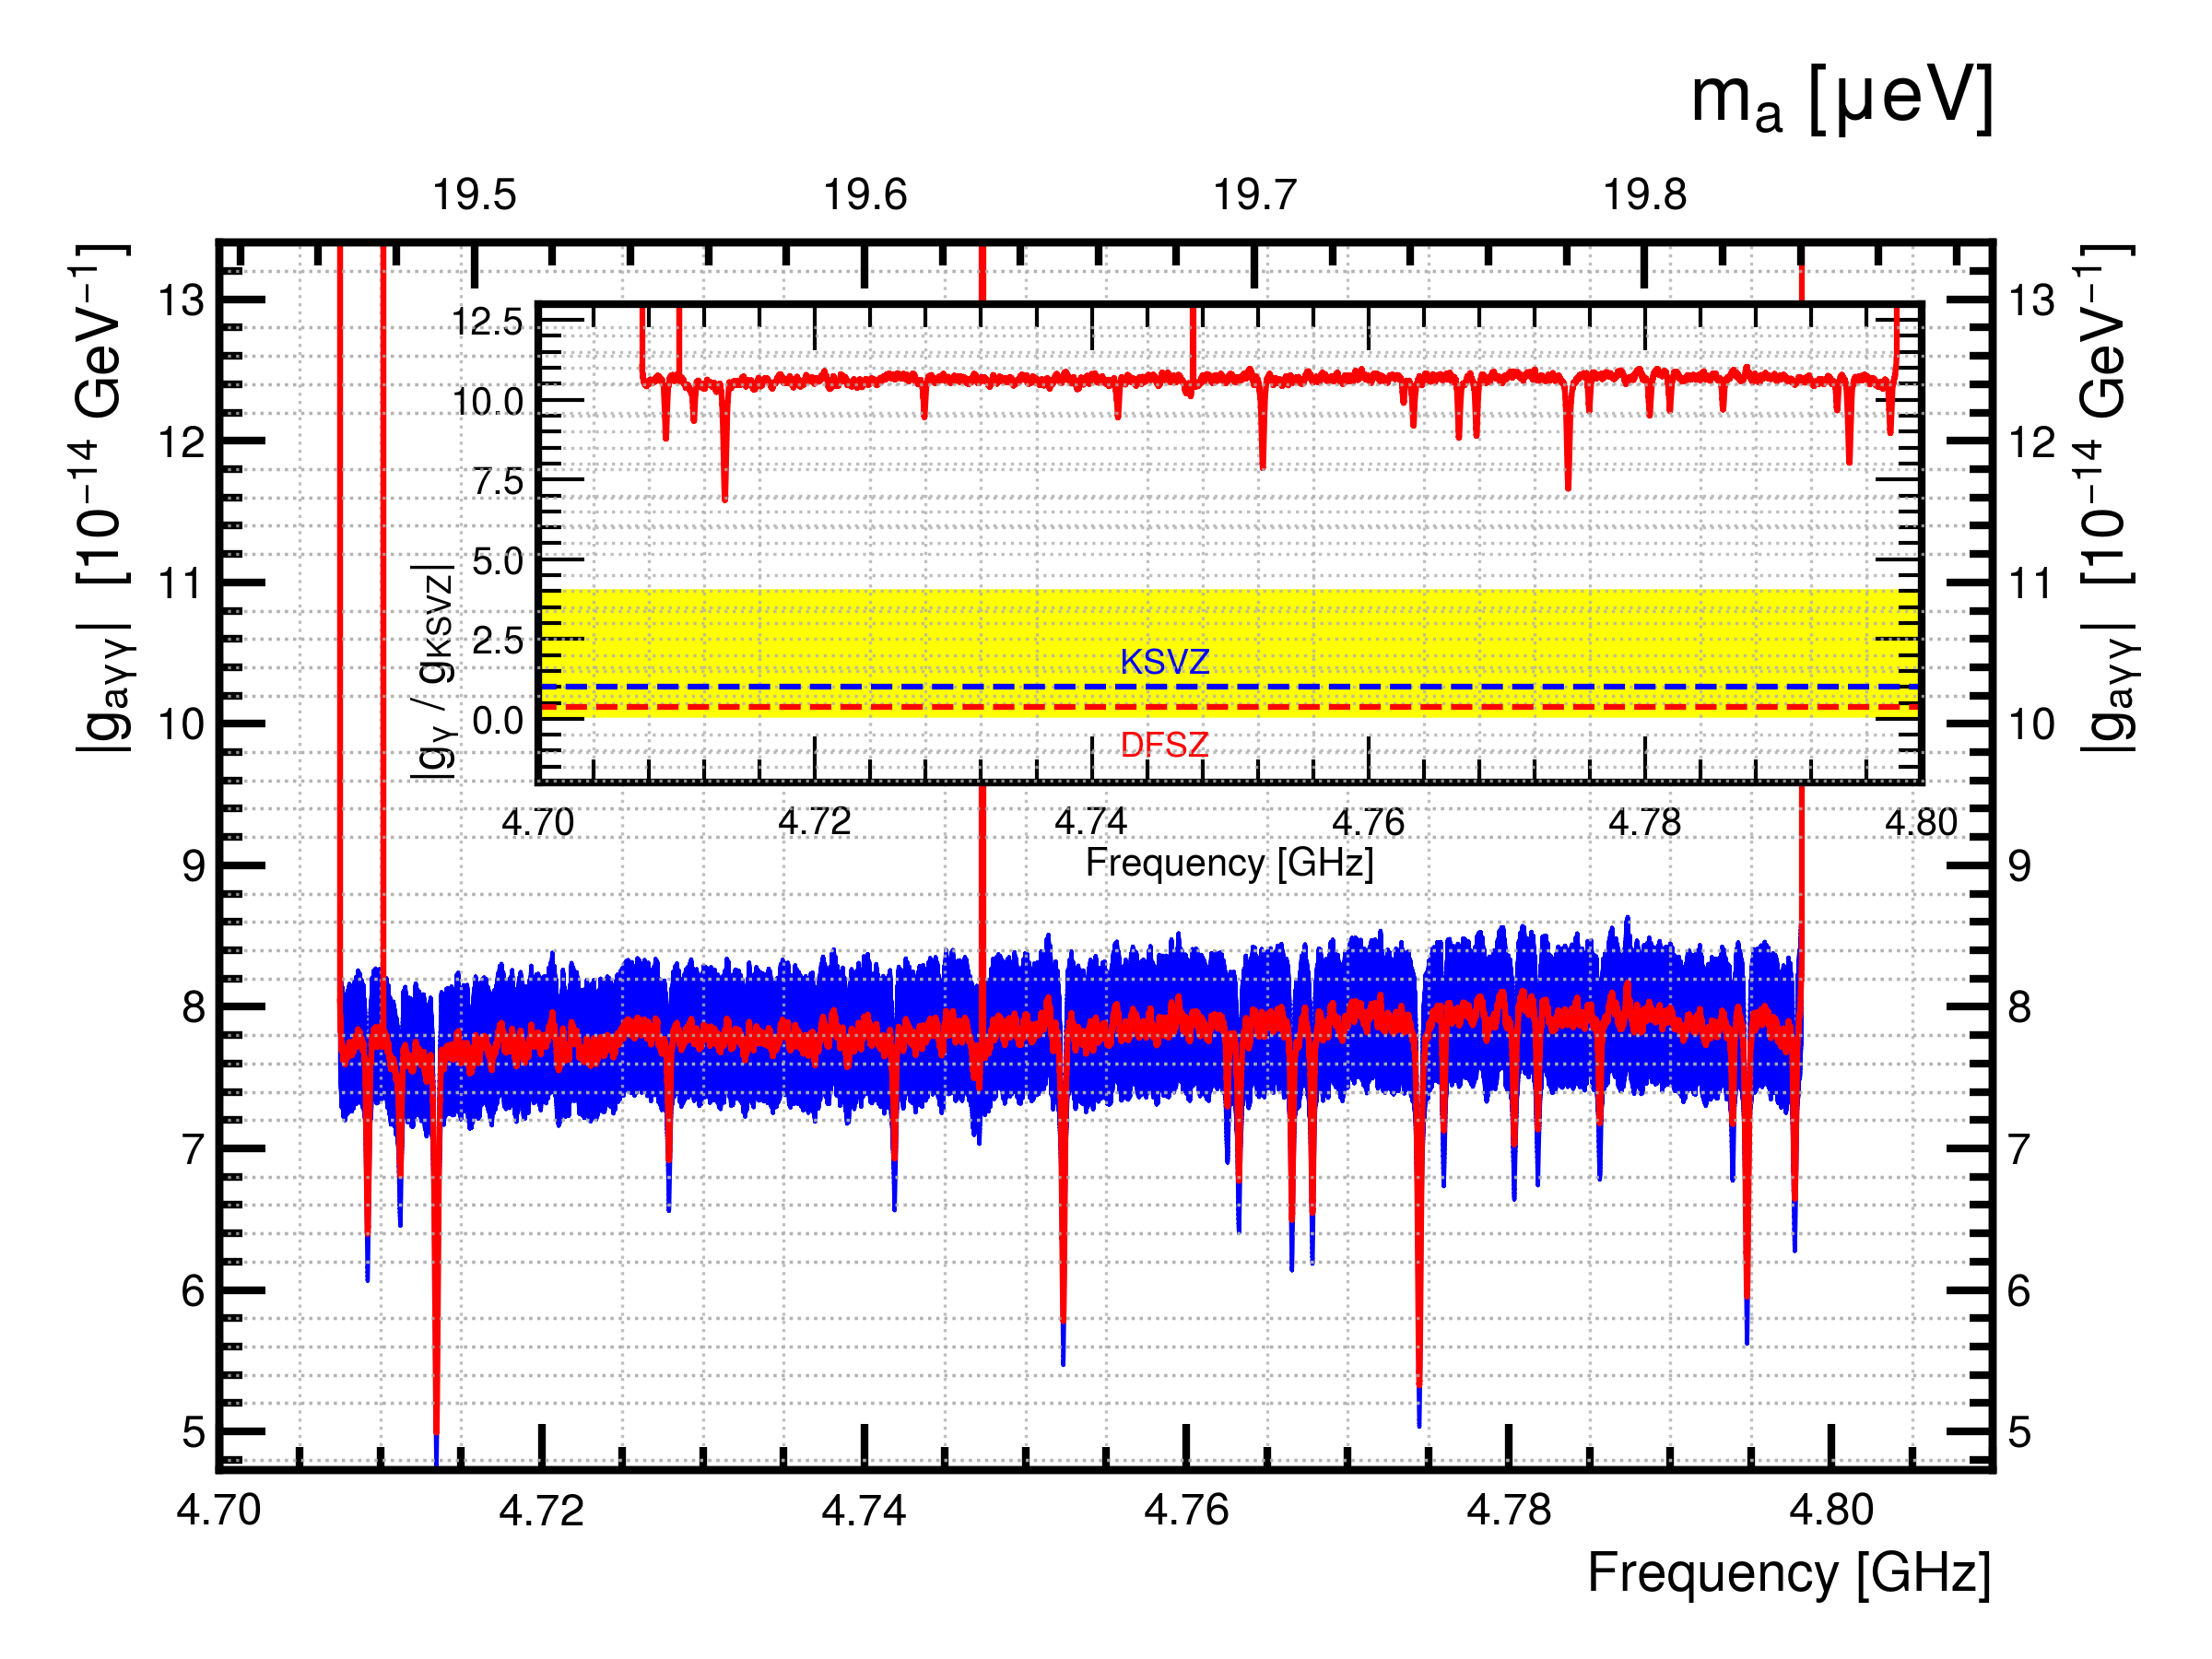
\includegraphics[width=12.9cm]{figures/TASEHonly_limits.png}
  \caption{The 95\% C.L. limits on \gagg\ and the ratio of the 
95\% C.L. limits on \ggamma\ relative to $\left|g_\text{KSVZ}\right|=0.97$ 
  (inset), for the frequency range of 
\flo--\fhi~GHz. The blue error band indicates the systematic 
  uncertainties as discussed in Sec.~\ref{sec:sys}. The yellow 
 band in the inset shows the allowed region of \ggamma\ vs. $m_a$ 
 from various QCD axion models, while the blue and red dashed lines are the 
values predicted by the KSVZ and DFSZ benchmark models, respectively.}
  \label{fig:glimit}
\end{figure*}


\begin{figure*} [htbp]
  \centering
 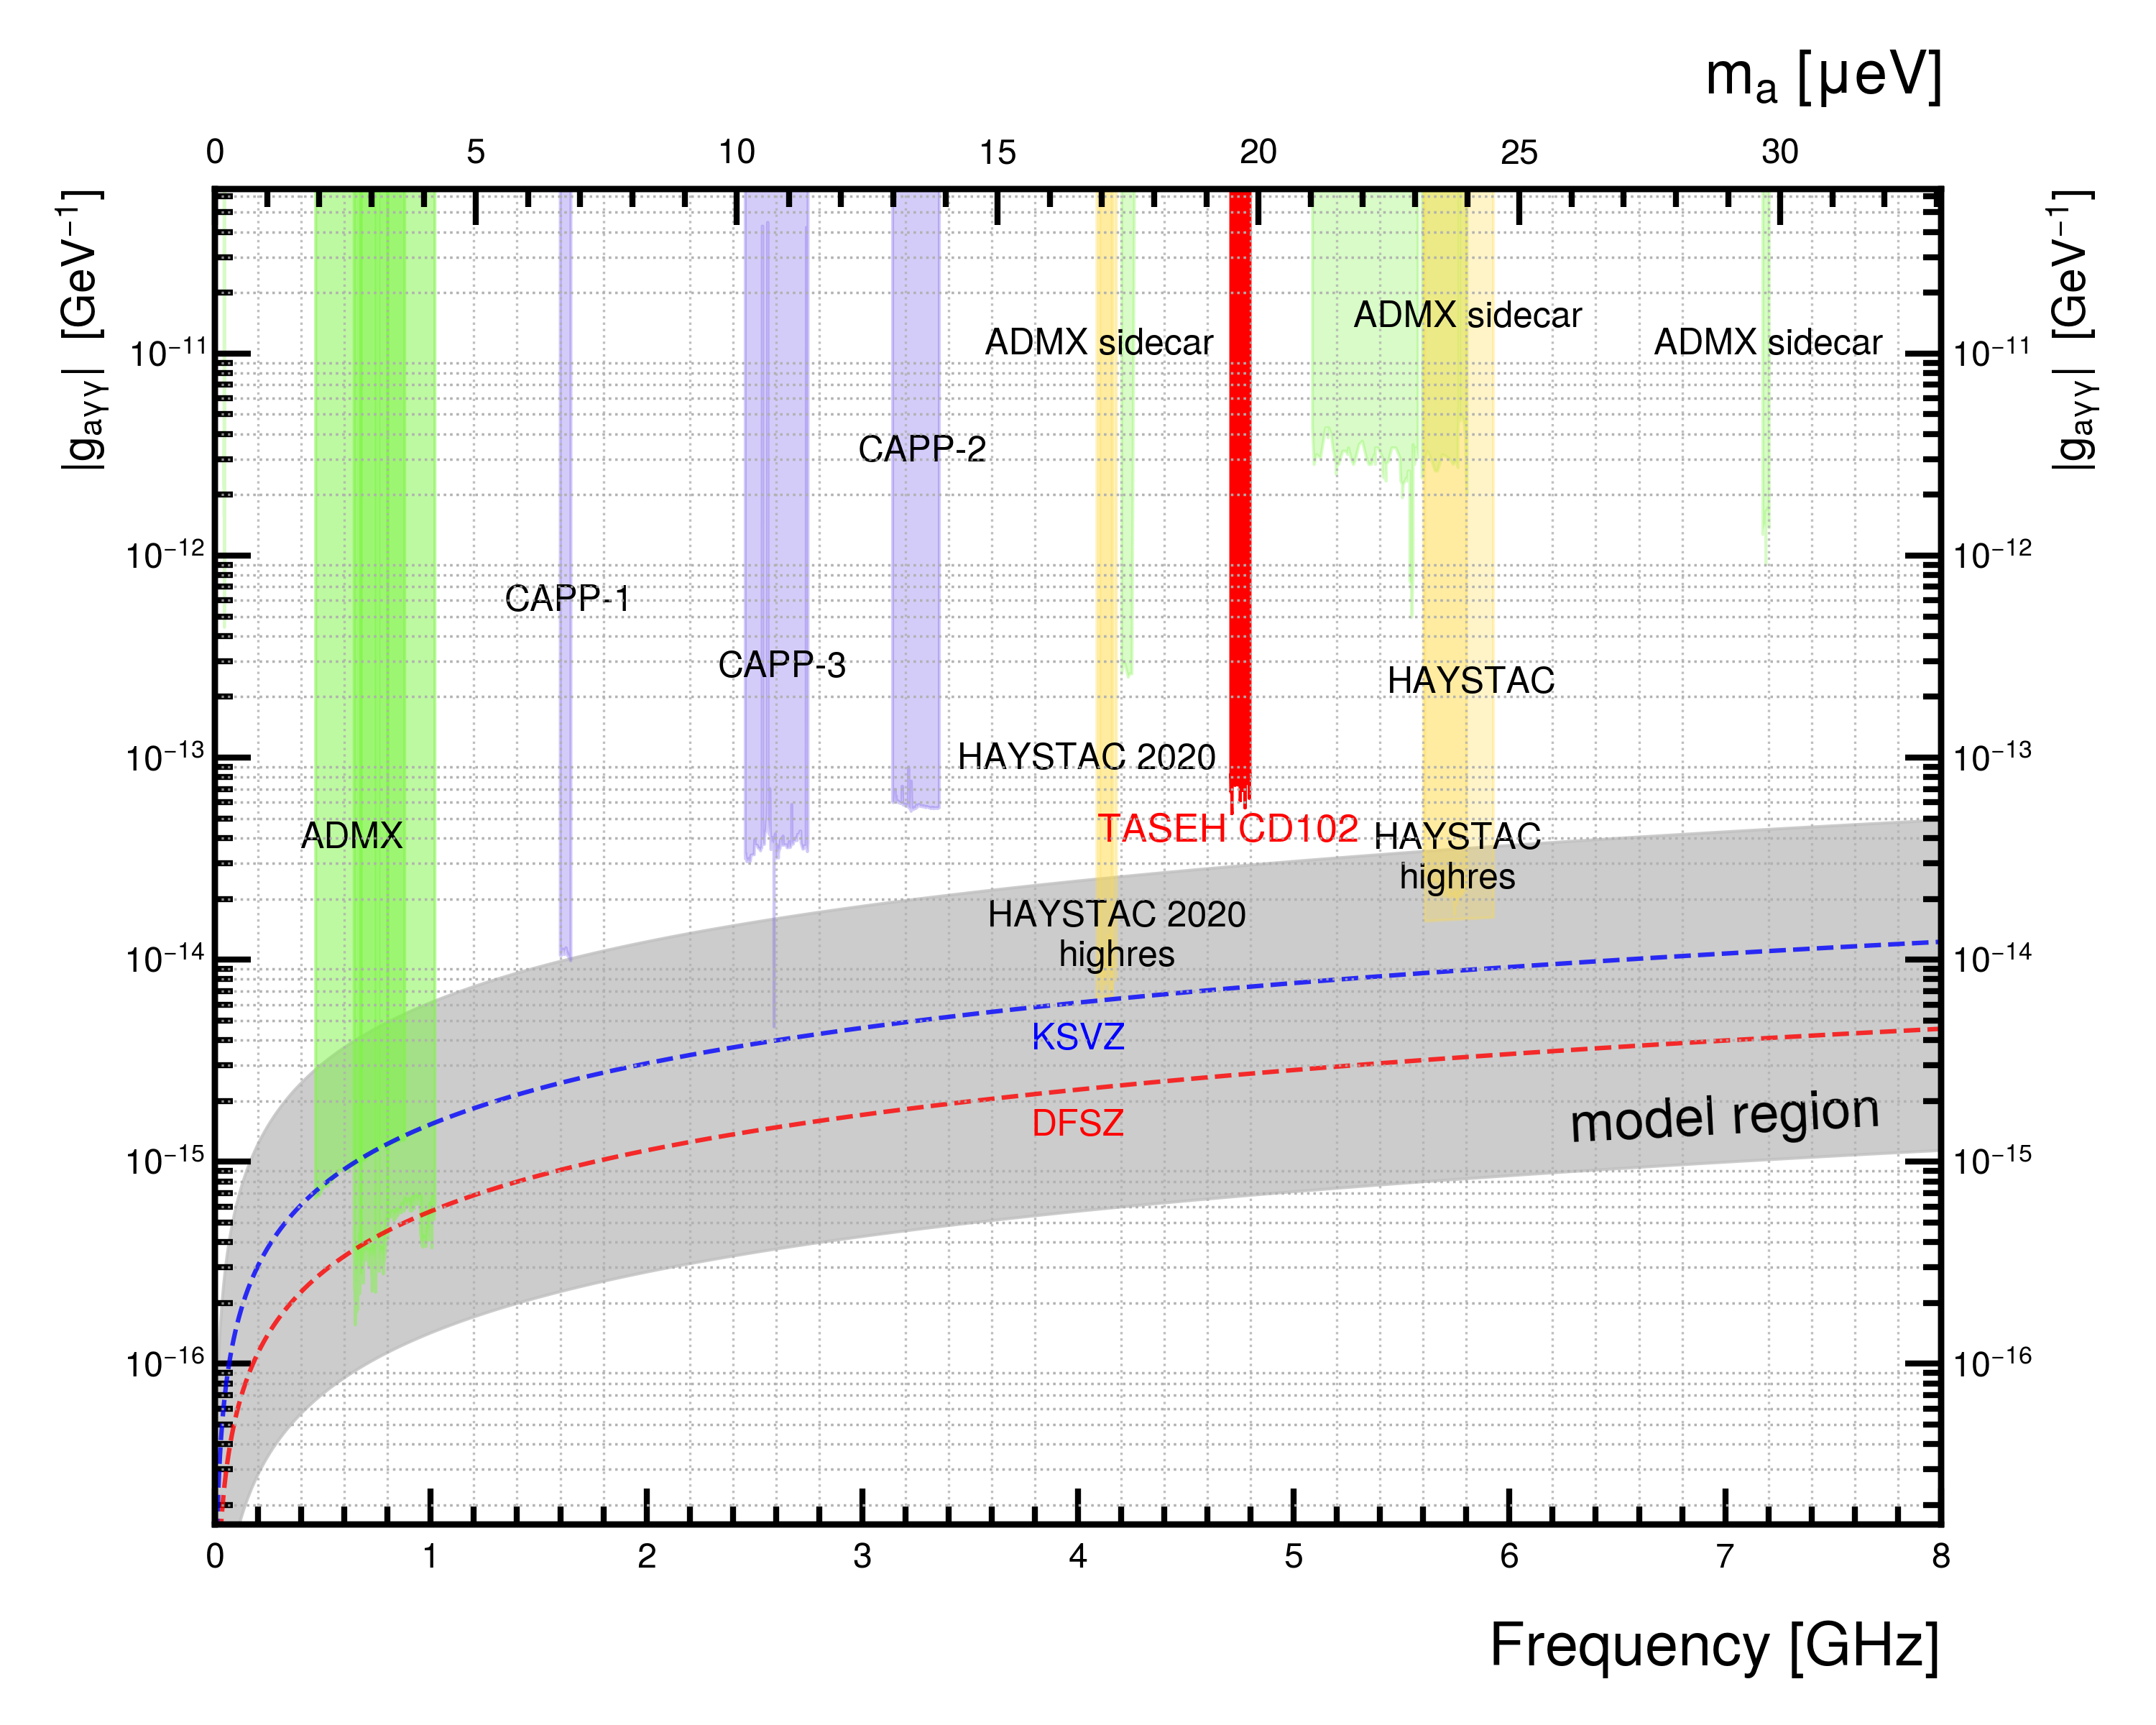
\includegraphics[width=12.9cm]{figures/RealData_limit_allexp.png}
  \caption{The limits on the axion-two-photon coupling \gagg\ for the 
frequency ranges of 0--8~GHz, from the CD102 data of TASEH (red band) and 
previous 
searches performed by the ADMX, CAPP, and HAYSTAC Collaborations. The gray 
band indicates the allowed region of \gagg\ vs. $m_a$ from various QCD axion 
models while the blue and red dashed lines are the values predicted by the 
KSVZ and DFSZ benchmark models, respectively.}
  \label{fig:gaggall}
\end{figure*}


